%%%%%%%%%%%%%%%%%%%%%%%%%%%%%%%%%%%%%%%%%
% Short Sectioned Assignment LaTeX Template Version 1.0 (5/5/12)
% This template has been downloaded from: http://www.LaTeXTemplates.com
% Original author:  Frits Wenneker (http://www.howtotex.com)
% License: CC BY-NC-SA 3.0 (http://creativecommons.org/licenses/by-nc-sa/3.0/)
%%%%%%%%%%%%%%%%%%%%%%%%%%%%%%%%%%%%%%%%%

%----------------------------------------------------------------------------------------
%	PACKAGES AND OTHER DOCUMENT CONFIGURATIONS
%----------------------------------------------------------------------------------------

\documentclass[paper=a4, fontsize=11pt]{scrartcl} % A4 paper and 11pt font size

% ---- Entrada y salida de texto -----

\usepackage[T1]{fontenc} % Use 8-bit encoding that has 256 glyphs
\usepackage[utf8]{inputenc}
%\usepackage{fourier} % Use the Adobe Utopia font for the document - comment this line to return to the LaTeX default

% ---- Idioma --------

\usepackage[spanish, es-tabla]{babel} % Selecciona el español para palabras introducidas automáticamente, p.ej. "septiembre" en la fecha y especifica que se use la palabra Tabla en vez de Cuadro

% ---- Otros paquetes ----

\usepackage{amsmath,amsfonts,amsthm} % Math packages
%\usepackage{graphics,graphicx, floatrow} %para incluir imágenes y notas en las imágenes
\usepackage{graphics,graphicx, float} %para incluir imágenes y colocarlas

% Para hacer tablas comlejas
%\usepackage{multirow}
%\usepackage{threeparttable}

%\usepackage{sectsty} % Allows customizing section commands
%\allsectionsfont{\centering \normalfont\scshape} % Make all sections centered, the default font and small caps

\usepackage{fancyhdr} % Custom headers and footers
\usepackage{url}
\usepackage[hidelinks]{hyperref}
\pagestyle{fancyplain} % Makes all pages in the document conform to the custom headers and footers
\fancyhead{} % No page header - if you want one, create it in the same way as the footers below
\fancyfoot[L]{} % Empty left footer
\fancyfoot[C]{} % Empty center footer
\fancyfoot[R]{\thepage} % Page numbering for right footer
\renewcommand{\headrulewidth}{0pt} % Remove header underlines
\renewcommand{\footrulewidth}{0pt} % Remove footer underlines
\setlength{\headheight}{13.6pt} % Customize the height of the header

\DeclareOldFontCommand{\rm}{\normalfont\rmfamily}{\mathrm}
\DeclareOldFontCommand{\sf}{\normalfont\sffamily}{\mathsf}
\DeclareOldFontCommand{\tt}{\normalfont\ttfamily}{\mathtt}
\DeclareOldFontCommand{\bf}{\normalfont\bfseries}{\mathbf}
\DeclareOldFontCommand{\it}{\normalfont\itshape}{\mathit}
\DeclareOldFontCommand{\sl}{\normalfont\slshape}{\@nomath\sl}
\DeclareOldFontCommand{\sc}{\normalfont\scshape}{\@nomath\sc}
\DeclareRobustCommand*\cal{\@fontswitch\relax\mathcal}
\DeclareRobustCommand*\mit{\@fontswitch\relax\mathnormal}

\numberwithin{equation}{section} % Number equations within sections (i.e. 1.1, 1.2, 2.1, 2.2 instead of 1, 2, 3, 4)
\numberwithin{figure}{section} % Number figures within sections (i.e. 1.1, 1.2, 2.1, 2.2 instead of 1, 2, 3, 4)
\numberwithin{table}{section} % Number tables within sections (i.e. 1.1, 1.2, 2.1, 2.2 instead of 1, 2, 3, 4)

\setlength\parindent{0pt} % Removes all indentation from paragraphs - comment this line for an assignment with lots of text

\newcommand{\horrule}[1]{\rule{\linewidth}{#1}} % Create horizontal rule command with 1 argument of height




%----------------------------------------------------------------------------------------
%	TÍTULO Y DATOS DEL ALUMNO
%----------------------------------------------------------------------------------------

\title{	
\normalfont \normalsize 
\textsc{{\bf Visión por computador (2016-2017)} \\ Grado en Ingeniería Informática \\ Universidad de Granada} \\ [25pt] % Your university, school and/or department name(s)
\horrule{0.5pt} \\[0.4cm] % Thin top horizontal rule
\huge Memoria Práctica 1 \\ % The assignment title
\horrule{2pt} \\[0.5cm] % Thick bottom horizontal rule
}

\author{Ignacio Martín Requena} % Nombre y apellidos

\date{\normalsize\today} % Incluye la fecha actual

%----------------------------------------------------------------------------------------
% DOCUMENTO
%----------------------------------------------------------------------------------------
\usepackage{graphicx}
\usepackage{listings}
\usepackage{color}
\definecolor{gray97}{gray}{.97}
\definecolor{gray75}{gray}{.75}
\definecolor{gray45}{gray}{.45}
 

\lstset{ frame=Ltb,
     framerule=0pt,
     aboveskip=0.5cm,
     framextopmargin=3pt,
     framexbottommargin=3pt,
     framexleftmargin=0.4cm,
     framesep=0pt,
     rulesep=.4pt,
     backgroundcolor=\color{gray97},
     rulesepcolor=\color{black},
     %
     stringstyle=\ttfamily,
     showstringspaces = false,
     basicstyle=\small\ttfamily,
     commentstyle=\color{gray45},
     keywordstyle=\bfseries,
     %
     numbers=left,
     numbersep=15pt,
     numberstyle=\tiny,
     numberfirstline = false,
     breaklines=true,
   }
 


\lstdefinestyle{consola}
   {basicstyle=\scriptsize\bf\ttfamily,
    backgroundcolor=\color{gray75},
   }
 
\lstdefinestyle{C}
   {language=C,
   }



\begin{document}

\maketitle % Muestra el Título

\newpage %inserta un salto de página

\tableofcontents % para generar el índice de contenidos

\listoffigures

\newpage



%----------------------------------------------------------------------------------------
%	Cuestion 1
%----------------------------------------------------------------------------------------

\section{Apartado A}

\subsection{Enunciado}
Implementar una función de convolución (ejemplo, void my\_imGaussConvol(Mat\& im, Mat\& maskCovol, Mat\& out) ) debe ser capaz de calcular la convolución 2D de una imagen con una máscara.\\
Ahora supondremos que la máscara es extraída del muestreo de una Gaussiana 2D simétrica. Para ello implementaremos haciendo uso de las siguientes funciones auxiliares ( 2 puntos):\\


1).- Calculo del vector máscara: Usar la función getGausssianKernel() . Verificar el resultado mostrando los vectores obtenidos
2).- Calcular la convolución de una imagen con una máscara gaussiana, usar filter2d(). Verificar el resultado mostrando resultado sobre distintas imágenes con distintos valores de sigma.
\subsection{Comentarios sobre el desarrollo}

En primer lugar leemos la imagen a la cual le calcularemos la convolución:

\begin{figure}[h]
\centering
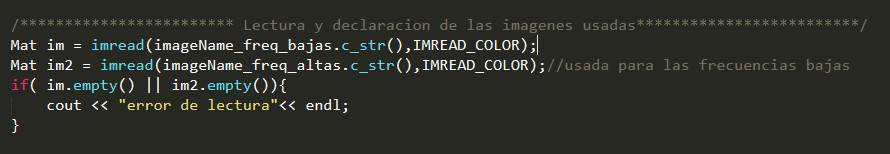
\includegraphics[width=0.7\linewidth]{lecturaimagen}
\caption{Lectura de la imagen}
\label{fig:lecturaimagen}
\end{figure}

Una vez cargada la imagen procedemos a calcular su convolución 2D. El procedimiento seguido ha sido:

\begin{itemize}
  \item \textbf{Calculamos la máscara para las frecuencias bajas.}
  
  Con la función \textit{getGaussianKernel} que nos proporciona OpenCv determinamos los valores de sigma y delta. En nuestro caso el valor de sigma viene determinado por un iterador que va aumentando en 20 unidades a fin de observar posteriormente los cambios de la imagen en función del parámetro sigma
  
  \item\textbf{ Hacemos una llamada a la función my\_imGaussConvol.}
  
  Esta función recibe como parámetros de entrada una imagen, una máscara calculada previamente y una imagen de salida donde se almacenará la imagen convolucionada.
  
  Los pasos para calcular la imagen convolucionada han sido:
  
  \begin{itemize}
  	\item En primer lugar damos la vuelta a la máscara con la función \textit{flip()}. Realmente este paso para nuestra máscara no sería necesario ya que al ser gaussiana esta es simétrica.
  	
  	\item Con la función \textit{filter2D} de OpenCV realizamos el filtado gaussiano de la imagen original con la máscara gaussiana.
  	
  	\item filter2D hace el filtrado en una única componente (en este caso la componente Y), por tanto debemos realizar un filtrado también en el sentido del eje X. Para ello trasponemos la imagen con el primer filtro pasado y volvemos a realizarle un segundo filtro igual al anterior
  	
  	\item Por último volvemos a trasponer la imagen final para que quede bien orientada
  \end{itemize}
  
  \item Acabamos mostrando la imagen por pantalla en cada iteración de nuestro bucle for
  
  
\end{itemize}

\subsection{Salidas obtenidas}

\begin{figure}[H]
\centering
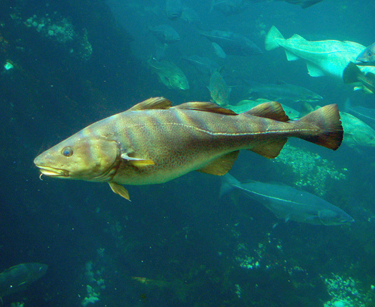
\includegraphics[width=0.5\linewidth]{a1}
\caption{Imagen con sigma = 1}
\label{fig:a1}
\end{figure}

\begin{figure}[H]
	\centering
	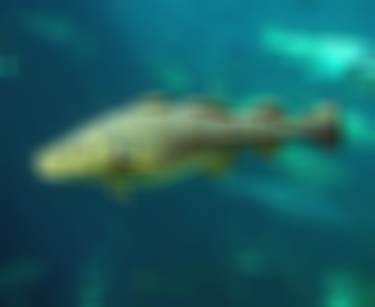
\includegraphics[width=0.5\linewidth]{A2}
	\caption{Imagen con sigma = 21}
	\label{fig:a2}
\end{figure}

\begin{figure}[H]
	\centering
	
\includegraphics[width=0.5\linewidth]{a3}
	\caption{Imagen con sigma = 41}
	\label{fig:a3}
\end{figure}

\begin{figure}[H]
	\centering
	
\includegraphics[width=0.5\linewidth]{a4}
	\caption{Imagen con sigma = 61}
	\label{fig:a4}
\end{figure}

Como podemos ver a mayores valores de sigma mayor número de frecuencias altas desechamos. Esto es debido principalmente a que con valores de sigma altos lo que hacemos es aumentar el tamaño de la máscara s y por tanto tengamos en cuenta un mayor numero de vecinos a la hora de hacer el filtro gaussiano.

\newpage
\section{Apartado B}

\subsection{Enunciado}

Mezclando adecuadamente  una parte de las frecuencias altas de una  
imagen con una parte de las frecuencias bajas de  otra imagen,  obtenemos una imagen híbrida que admite distintas interpretaciones a  distintas distancias ( ver hybrid images project page).\\
\\   
Para seleccionar la parte de frecuencias altas  y bajas que nos quedamos  de cada una de las imágenes usaremos el parámetro sigma del   núcleo/máscara de alisamiento gaussiano que usaremos. A mayor valor  
de sigma mayor eliminación de altas frecuencias en la imagen  
convolucionada. Para una buena implementación elegir dicho valor de  forma separada para cada una de las dos  imágenes ( ver las  
recomendaciones dadas en el paper de Oliva et al.). Recordar que las  máscaras 1D siempre deben tener de longitud un número impar.\\   

Usar la convolución que hemos implementado en el apartado A para  elegir los sigmas más adecuados para la selección de frecuencias en  parejas de imágenes ( ver fichero de datos). \\ 
1.   Implementar una función que genere las imágenes de baja y  
alta frecuencia.\\ 
2.   Escribir una función para mostrar las tres imágenes ( alta,  
baja e híbrida) en una misma ventana. (Recordar que las  
imágenes después de una convolución contienen número  
flotantes que pueden ser positivos y negativos)

\subsection{Comentarios sobre el desarrollo}

Una imagen híbrida es la combinación de dos imágenes, una que posee mayormente frecuencias bajas y otra que posee mayormente frecuencias altas.\\ 
\\
La característica más notable de este tipo de imágenes es que a tamaños de imagen grandes y observándola relativamente cerca podemos percibir fácilmente las frecuencias altas, mientras que con tamaños de imagen pequeños o viéndola desde la lejanía nuestro ojo percibe prácticamente sólo frecuencias bajas. Por tanto, una vez obtenida la imagen híbrida y ajustados los valores de sigma de cada una de las dos imágenes deberíamos experimentar este efecto.\\
\\

El cálculo de la imagen hibrida se ha realizado siguiendo los siguientes pasos:

\begin{itemize}
	\item {En primer lugar, a partir de la imagen que usaremos para las frecuencias bajas calculamos su convolución aplicando un kernel gaussiano (ver apartado A).}
	
	\begin{figure}[H]
		\centering
		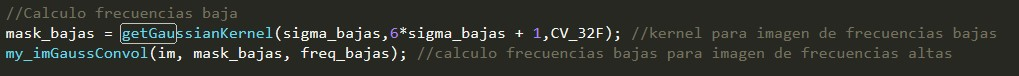
\includegraphics[width=0.6\linewidth]{freq_bajasB}
		\caption{Código frecuencias bajas }
		\label{fig:freq_bajasB}
	\end{figure}
	
	El valor de sigma en este caso depende de la imagen de entrada, por lo que se ha ajustado para cada una de las imágenes posibles un valor de sigma correcto para poder percibir el efecto explicado anteriormente.
	
	\item A continuación calculamos las frecuencias altas de una imagen.
	
	Para ello en primer lugar calculamos su filtro gaussiano y una vez obtenido restamos a la imagen original los valores de frecuencia bajas obtenidos en el filtro gaussiano:
	
		\begin{figure}[H]
			\centering
			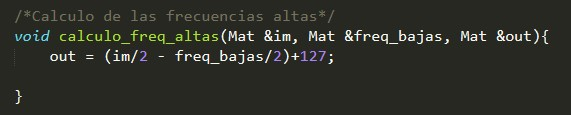
\includegraphics[width=0.6\linewidth]{freq_altasB}
			\caption{Cálculo frecuencias altas }
			\label{fig:freq_altasB}
		\end{figure}
		
		Como vemos, el calculo es una simple resta de cada valor de la imagen original con la de frecuencias altas y su posterior normalización para que los valores finales estén dentro del rango [0-254]
		
	\item Una vez calculada la imagen de alta frecuencia tenemos lo necesario para obtener nuestra imagen hibrida de la siguiente forma:
	
	\begin{figure}[H]
		\centering
		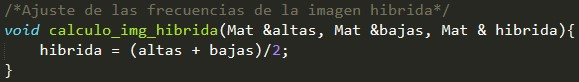
\includegraphics[width=0.6\linewidth]{calculo_hibrida}
		\caption{Cálculo frecuencias altas }
		\label{fig:freq_altasB}
	\end{figure}
	
	Cuya operación no es más que una suma de los valores calculados de la imagen de alta y la de baja frecuencia y su posterior nacionalización
	
	\item Para terminar concatenamos las imágenes de alta y baja frecuencia junto con la híbrida con la función \textit{hconcat} de OpenCV.
\end{itemize}

\subsection{Salidas obtenidas}

\begin{figure}[H]
	\centering
	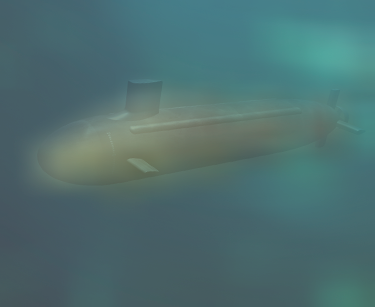
\includegraphics[width=0.6\linewidth]{b2}
	\caption{Imagen frecuencias bajas}
	\label{fig:freq_altasB}
\end{figure}

\begin{figure}[H]
	\centering
	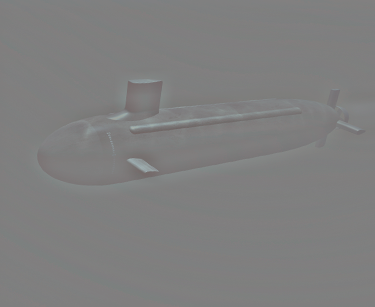
\includegraphics[width=0.6\linewidth]{b1}
	\caption{Imagen frecuencias altas }
	\label{fig:freq_altasB}
\end{figure}

\begin{figure}[H]
	\centering
	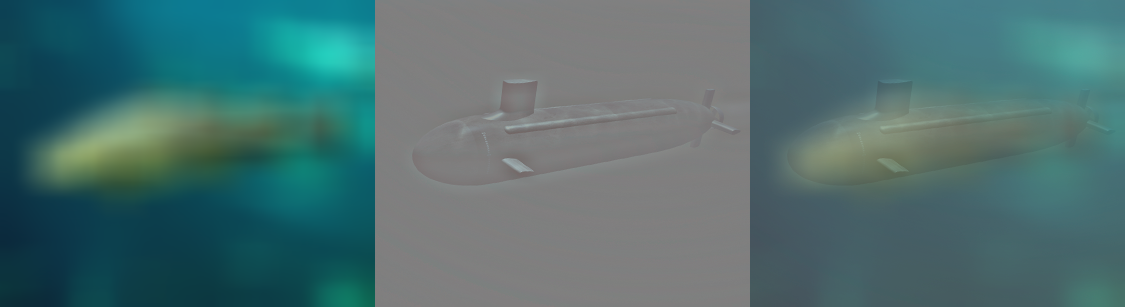
\includegraphics[width=1\linewidth]{b3}
	\caption{Concatenación de la imagen de frecuencias bajas, altas e imagen híbrida}
	\label{fig:freq_altasB}
\end{figure}

Como podemos observar la imagen híbrida cumple la propiedad comentada al inicio del apartado

\newpage
\section{Apartado C}

\subsection{Enunciado}

Construir una pirámide Gaussiana  de al menos 5 niveles con las  
imágenes híbridas calculadas en el apartado anterior.  Mostrar los  distintos niveles de la pirámide en un único canvas e interpretar el  resultado. 

\subsection{Comentarios sobre el desarrollo}
La representación en forma de pirámide de una imagen híbrida nos da una idea de si los valores de sigma elegidos en el calculo de las imágenes de alta y baja frecuencia son los adecuados o no sin necesidad de estar continuamente alejándose y acercándose del monitor para comprobarlo.\\
\\
Esta imagen piramidal se compone un número determinado de niveles. En cada nivel se aloja una imagen híbrida resultado de reducir su tamaño a la mitad de la que le precede, así que lo lógico es calcular todas las reducciones de las imágenes según el número de niveles. Esto se ha hecho de la siguiente forma:

\begin{figure}[H]
	\centering
	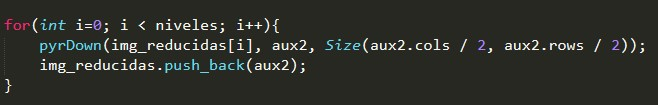
\includegraphics[width=1\linewidth]{imagenes_reducidas}
	\caption{Cálculo de la reducción del tamaño de la imagen híbrida}
	\label{fig:freq_altasB}
\end{figure}

En un vector de tipo Mat vamos almacenando la reducción a la mitad del tamaño de la imagen anterior tantas veces como número de niveles deseemos en nuestra pirámide.

Una vez calculadas estas imágenes debemos ajustar el tamaño de las mismas para que \textquotedblleft cuadre \textquotedblright con el resto de imágenes ya que es imposible concatenar imágenes que tienen diferente número de filas (para concatenaciones en horizontal) o columnas (para concatenaciones en vertical). Para solventar este problema hacemos lo siguiente:

\begin{itemize}
	\item A los niveles que difieren en número de columnas con respecto a la imagen de nivel 1 (consideramos la imagen original el nivel 0 de la pirámide) les añadimos tantas columnas como le falten para que tenga las mismas que la de nivel 1 y rellenamos estas filas añadidas de negro:
	
	\begin{figure}[H]
		\centering
		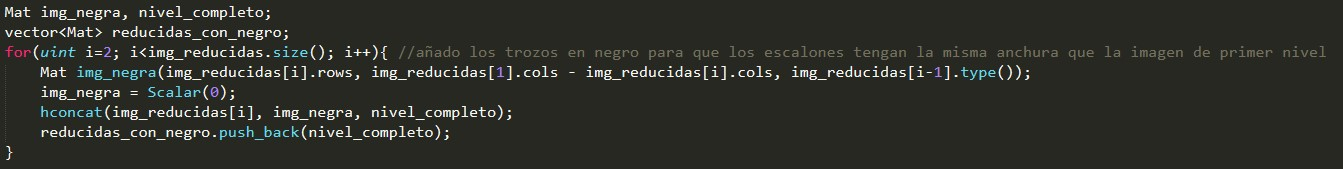
\includegraphics[width=1\linewidth]{niveles_negro}
		\caption{Ajuste tamaño de los niveles 2 a 5}
		\label{fig:freq_altasB}
	\end{figure}
	
	\item Concatenamos los niveles de todas las imágenes una vez generadas y ajustadas:
	
	\begin{figure}[H]
		\centering
		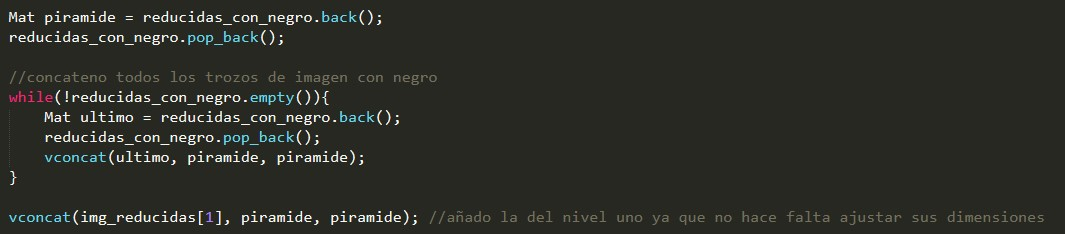
\includegraphics[width=1\linewidth]{concatenacion_niveles}
		\caption{Concatenación vertical de los niveles 1-5}
		\label{fig:freq_altasB}
	\end{figure}
	
	\item Por último, ajustamos el número de filas de la imagen concatenada en el punto anterior para que tenga el mismo tamaño que el de la original y concatenamos con esta:
	
		\begin{figure}[H]
			\centering
			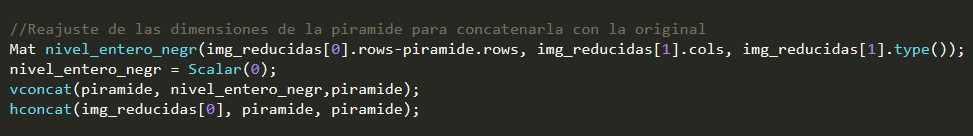
\includegraphics[width=1\linewidth]{niveles_original}
		\caption{Concatenación original con reducidas}
		\label{fig:freq_altasB}
	\end{figure}
	
	
\end{itemize}

\subsection{Salidas obtenidas}

		\begin{figure}[H]
		\centering
		
\includegraphics[width=1\linewidth]{nivel2pyr}
		\caption{Nivel 2 de la pirámide con el ajuste de dimensión}
		\label{fig:freq_altasB}
		\end{figure}
	
		\begin{figure}[H]
		\centering
		
\includegraphics[width=1\linewidth]{nivel3pyr}
		\caption{Nivel 3 de la pirámide con el ajuste de dimensión}
		\label{fig:freq_altasB}
		\end{figure}
	
		\begin{figure}[H]
		\centering
		
\includegraphics[width=1\linewidth]{nivel4pyr}
		\caption{Nivel 4 de la pirámide con el ajuste de dimensión}
		\label{fig:freq_altasB}
		\end{figure}
			
		\begin{figure}[H]
			\centering
			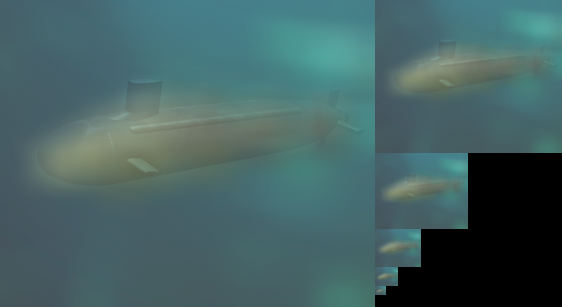
\includegraphics[width=1\linewidth]{piramide}
			\caption{Resultado final de la pirámide}
			\label{fig:freq_altasB}
		\end{figure}

Como podemos comprobar, por debajo del nivel 2 vemos mayormente un pez (imagen con bajas frecuencias) y en los niveles 1 y 2 observamos mejor el submarino (imagen con frecuencias altas).
\end{document}